\documentclass{article} % This line defines the type of document. 'article' is a common class for small documents.
\usepackage[margin=1.4in]{geometry}
\usepackage{graphicx}
\usepackage{titlesec}

\titleformat{\section}
  {\normalfont\large\bfseries}{\thesection}{1em}{}

\begin{document} % This line marks the beginning of the document content.


\noindent\makebox[\linewidth]{\rule{\textwidth}{1pt}} 
\vspace*{0mm} % adds vertical space before the title
\begin{center}
    \Large\textbf{Toy Models of Superposition Replication and Findings}
\end{center}
\vspace*{2mm} % adds vertical space before the title
\noindent\makebox[\linewidth]{\rule{\textwidth}{1pt}}
\newline

\begin{abstract}
\begin{quote}
    Toy Models of Superpostion\cite{elhage2022toy} is a groundbreaking paper published by 
    researchers affilated with Anthropic and Harvard University in 2022. The
    paper demonstrates that neural networks can represent more features than
    they have demensions buy training small models with under 100 neurons. Additionally,
    they use these so called "toy models" to understand the relationship between
    how neural networks are trained and how they represent the data internally.
    This paper was able to the finding from this paper and make new observations
    about "toy models" and how they behave under different training circumstances.
\end{quote}
\end{abstract}


\section{Background and Motivation}


\begin{figure}[h]
    \centering
    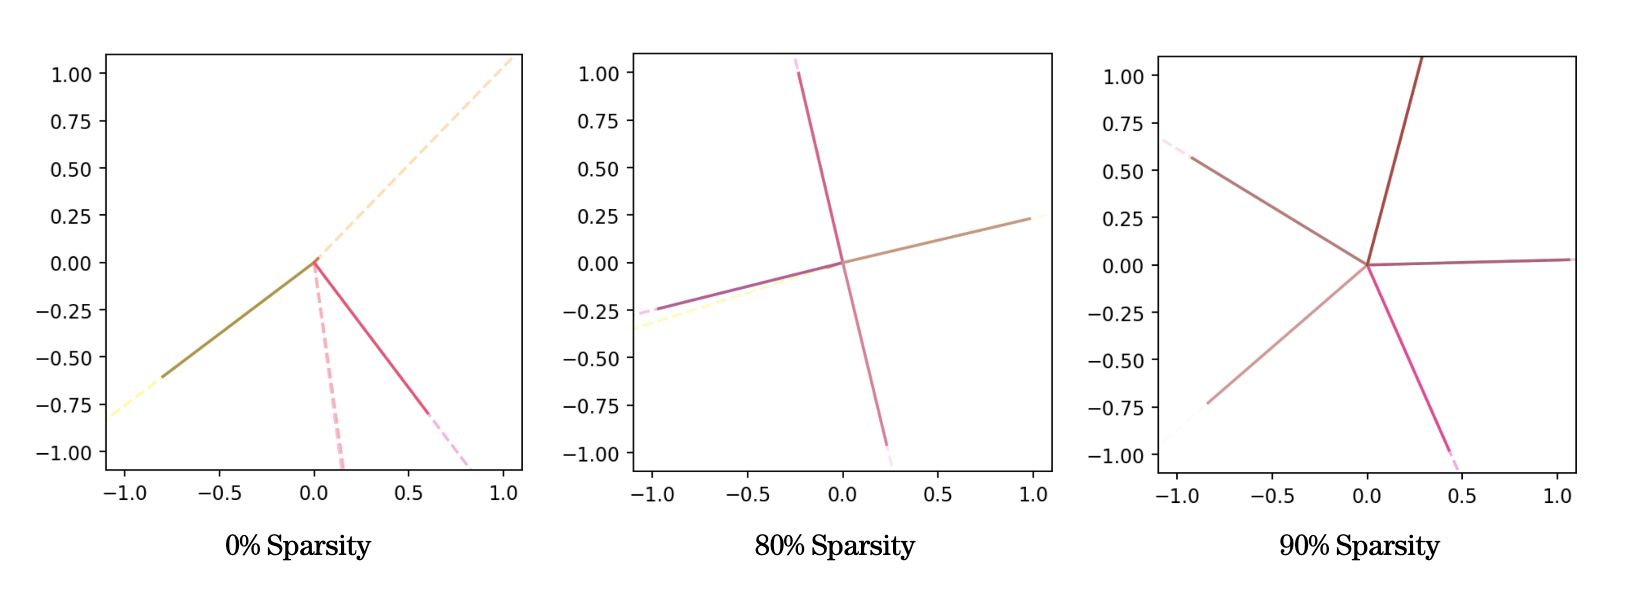
\includegraphics[width=0.7\linewidth]{section_1/images/section1_replicated_graphic.png}
    \caption{Replicated feature directions example.}
    \label{fig:section1_replication}
\end{figure}

\begin{figure}[h]
    \centering
    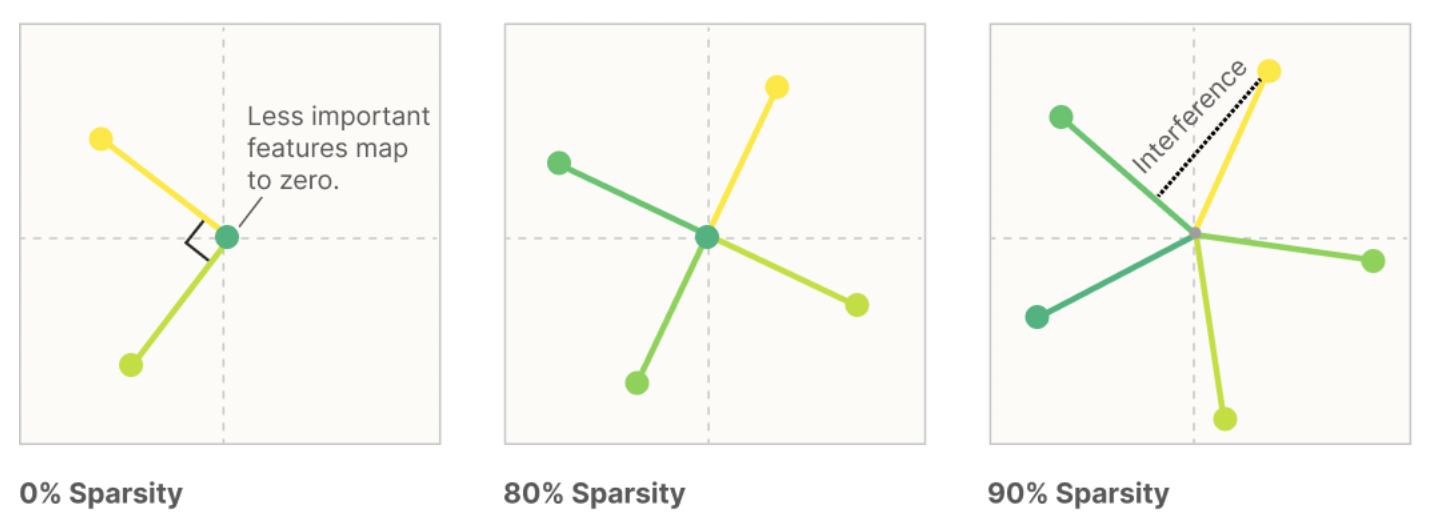
\includegraphics[width=0.67\linewidth]{section_1/images/section1_anthropic_graphic_.png}
    \caption{Graphic from Anthropic Paper}
    \label{fig:section1_anthropic}
\end{figure}

\section{Demonstrating Superposition}

In this section of Toy Models of Superpostion\cite{elhage2022toy}, the researchers
provide context and define terms. This provides a good overveiw for people
unfamiliar with some of the concepts discussed in this replication.\newline\newline
In this paper, I make a few additional comments about some key terms to provide
context in this paper. \newline \newline
\textbf{(1) Defining Features: }The original paper Toy Models of Superpostion
defines features broadly as "properties of the input which a sufficiently large 
neural network will reliably dedicate a neuron to representing." The authors do
however describe this definition as "slightly circular" and note that they are
not "overly attached to it."\newline\newline
I find the definition especially problematic because a network that is small or
has unconventional archetecture may represent a feature that a larger network
or a network with a more typical archetecture may represent. In other words, just
because a nueral network represents the input in a way that a "sufficiently large network"
would never represent, does not mean that we should not think of these representations 
as features.\newline\newline
As a result, I propose an alternative definition: features are aspects of the
input that a neural network represents accuratly with a higher propability than 
a randomly initialized network. In other words, features are parts of the input 
that a model determines to be important enough to represent internally.


\bibliographystyle{plain}
\bibliography{references}

\end{document} % This line marks the end of the document content.
